
\chapter{绪论}
\section{研究背景}

通信的主要目的是传达信息。 
无论是在传统的有线通信系统还是在无线通信系统中,由于信道传输特性的限制,
基带信号不能直接通过信道传输,而是需要对基带信号进行调制以将其搬移到 一定的频段进行有效的传输。 
同时,对基带信号的调制还可以使通信系统具有更高的传输速率并提高频谱利用率。\par

随着通信技术的不断发展,用户对于信息传输速率要求的不断提高,以及人们对于无线通信便利性的需求,
通信信号的调制形式由简单到复杂,调制方式由传统的模拟调制发展到主流的数字调制方式,
信道从有线信道到有线与无线信道混合组网。
模拟调制针对的是模拟信号,传统的模拟调制按照调制方式的不同,
可以将其分为幅度调制(AM)、频率调制(FM)和相位调制(PM)等;
数字调制针对的是数字信号,按照调制方式的不同可以分为
幅移键控(ASK)、频移键控(FSK)、相移键控(PSK)和正交幅度调制(QAM)等。 \par

通信技术的迅速发展导致了各种通信系统的共存。
 然而,这些通信系统的调制方式不同,各种调制技术也导致接收机类型大幅增加。
 于是,人们希望能够通过发展新的无线认知技术,基于通用的接收机平台来接收并识别不同的调制信号,
 以减少接收机类型的快速增长,提高通信设备的稳定性与通用性,降低建设与运维成本。 \par

调制方式是一种区分不同类型信号的重要特征。
所谓的调制方式自动识别,是指我们可以在未给定调制信号所携信息的情况下,通过接收信号电磁特性确定信号的调制方式;
并在非人工干预条件下,估计信号的相应调制参数。
在密集和复杂的多用户频谱环境中自动识别不同类别的调制信号,
是一种优化频谱利用效率,识别和最小化干扰,以及有效推动认知无线网发展的重要手段。
调制自动识别技术在军队和政府部门的无线电管理中也起着重要作用。
在军事领域,调制识别被广泛地用作通信侦察,电子战和威胁分析,是一种智能信号分析和处理的关键技术[9]。
在现代战争中,战场信息的传播主要依赖于无线通信,而侦察通讯信号则是电子战的主要内容。
在侦听接收机的设计中,获取无线接收信号的调制方式是侦听接收机的重要功能之一。
有效的无线信号调制方式识别为解调器正确选择解调算法提供了参数依据,可以使我们最终得到准确的情报信息。
调制识别技术也有助于为电子战选择最佳的干扰模式或干扰消除算法,以保证友好的通信,
同时抑制和干扰对方的通信以达到电子战通信对抗的目的。\par

另外,在自适应调制系统中发射信号的调制方式会随信道状态而变化。
接收端为了正确解调信号,就需要知道发射信号的调制信息。
发送信令是最简单的方式,即通过在一个包发送含有调制信息的控制信号到接收机,接收机对其进行解调就可以获得信号的调制方式。
但是这种方式是以牺牲有用信息的带宽为代价的;
如果发射信号中不包含调制参数信息,则可以减小带宽开销。
这就需要我们利用调制识别技术对接收信号进行判别,获取其调制类别参数,对信号进行解调。\par

因此,通信信号调制自动识别技术具有非常广阔的应用前景,将成为现代战争通信和未来无线通信应用的重要组成部分。\par

深度学习(Deep Learning,DL),是一种在很多工业应用中具有最高分性能的机器学习(Machine Learning,ML)领域的分支[1]。 
2007年在NetFlex的推荐比赛中,XX凭借深度玻尔兹曼机(Deep Bolzman Machine,DBM)获得冠军,开启了最近的一波深度学习浪潮。
在2012年的ImageNet大规模视觉识别挑战赛(ILSVRC)中,Alex凭借对于卷积神经网络的改进,
提出的AlexNet网络框架【】,以超出第二名20\%多的极大优势夺得冠军。
在ImageNet2014中,谷歌提出了(Inception Model)获得了冠军,在ImageNet2015中,微软凭借(ResNet)夺得冠军,
在ImageNet2016中,海康威视凭借改进的200多层的模型取得冠军,从最近的几年来看,夺冠的前几名,无一例外使用深度学习模型,
获得了ImageNet比赛的冠军,并且已经远远地超过了人类专家所能达到的最高分类能力。
在NLP领域,Google提出的Word2Vec极大地提高的翻译的准确度,在推荐领域,Youtube的Word2Vec模型受到了广大互联网公司的争相借鉴。
DeepMind提出的基于深度学习与增强学习的Zero,在2017年击败了柯洁,我们在最引以为傲的围棋领域也被人工智能(Artificial Intelegence)击败。
在医学领域,深度学习也被广泛的研究应用于医学影像处理;在生物学领域,深度学习也被应用于人类基因的处理, 从DNA序列中找到连接。
尽管一些传统的ML算法如支持向量机(SVM)和K近邻(KNN)已被用于媒体访问控制(MAC)、协议识别[5]、调制分类[6]等,
但是DL在通信中的使用却相对较少。\par

在通信系统中使用DL有几个优点。 
首先,由于通信基础设备以及终端的数量多,且通信数据速率高,因此可以很容易获取DL训练所需要的大量数据。
其次,DL可以自主提取特征,避免了手动特征选择这一繁琐且具有挑战性的任务。
第三,由于DL正在迅速发展,除了调制分类之外,其他通信应用将具有相当大的潜力,可以提升我们传统方法的性能上界。
另外,新的、更复杂的信号和通信应用的出现,给认知无线带来了更大的挑战;
有时,我们需要对一些未知的信号进行认知,而传统的基于特征的方法在新的场景下很难适应信号特性的变化。
因此,我们可以利用深度学习的特征自提取能力,来增强对于未知信号的认知能力。\par


\section{研究意义}

在无线通信中,调制识别是正确实现无线通信解调和保证正常接收的重要组成部分。
基带信号通常是频率非常低且分量很多的频谱,这些含有很多低频分量的信号不适合在信道中直接传输,
这就需要我们对基带信号进行调制,以适应信道的特性并在无线信道中进行有效传输。
信号在经过调制并通过信道到达接收端,与原始的信号具有很大的不同。
所以,只有在接收端确定信号的调制方式,才能利用相应的解调方法解调获取原始信息。\par

\subsection{调制识别的意义}
在民用通信中,对于一些非合作性的通信,
政府无线电管理部门需要对民用通信信号进行监控与管理,必要时还需要进行侦听与拦截。
在这种情况下,由于管理与被管理双方通信未必事先预定,
通信的调制方式类型的识别、载波频率、波特率及其它调制参数的正确估计变得尤为重要。\par

在军事训练中的电子对抗、电磁干扰与反干扰中,当检测到对方无线电信号或电磁信号时,
需要我们对检测到的信号或电磁信息进行调制识别以及载玻频率与波特率的正确估计等,
以便进一步侦听破译对方通信情报信息或者对对方进行高强度的无线电干扰或者电磁干扰,
使对方无线通信受到阻碍甚至中断。\par

在认知无线领域,当前的无线频谱资源根据具体业务的不同,
主要划分为民用的广播电视、无线通信、卫星通信及军用的雷达与军事通信等不同频段。
为了避免相邻频段或频道的互相干扰,不同的通信业务的工作频段相互隔离,
并且不同频段之间预留一定的间隔频带;
上下频段的频谱资源分配以及频谱利用率极不平衡,造成了频谱资源的极大浪费。
随着频谱资源的消耗殆尽,现有的频谱分配与管理机制已经成为制约无线通信进一步发展的重要因素。
因此,如何在现有无线频谱资源基础上,如何在频域、时域和空域等多维度上有效分配频谱资源,
提高频谱利用率,已经成为认知无线亟需解决的问题。\par

\subsection{深度学习与无线通信的结合}

无线通信是一个特定的信号处理领域。 
在这个领域中,经过多年的积累,利用专家特征和判决准则进行调制识别得到了广泛的应用,并且在特定情况下可以实现很高的识别准确率。
然而,通过深度学习在图像、NLP、推荐系统等领域的突破性进展以及广泛应用,
很多基于深度学习的方法已经提高了传统机器学习算法的上限,甚至超过了人类专家在相应领域的辨识与认知能力。\par

应用于图像处理[11]和语音识别[18]的深度学习方法绝大多数是基于数据进行特征学习,而不是利用专家特征进行训练,
这与很多传统的机器学习算法(比如DNN、SVM、决策树等)有很大不同。
因此,对于认知无线领域的一些传统应用,需要我们重新审视一下是否也应该对传统的学习算法进行相应的思路转变。\par

同时,深度学习在通信领域的应用,也带来了新的机遇与变革,XXX等人利用深度学习进行半监督识别,
有效的利用了无监督数据,XXX等人将深度学习应用于路由,提高了识别准确率等。
深度学习在通信领域也已经得到了初步的应用,并取得了一定的成果。但是这些应用大都是一些验证性的应用,
并没有进行深入的研究。\par

因此,需要我们进一步探索什么样的深度网络结构适应哪一些特定的领域,
在具体问题中影响深度学习算法性能的因素是什么,如何改进深度学习的算法框架以提高我们模型的性能,
如何将过去几十年的研究成果与深度学习相结合等等。\par

\section{无线信号调制识别的发展和研究现状}

早期调制识别的任务是由操作人员在仪器的帮助下完成的:
主要是通过观察和分析接收信号的时域波形和频谱形状,判断信号的调制方式,然后选择相应的解调器进行解调。
然而,随着无线通信技术尤其是数字通信技术的快速发展,信号调制方式变得越来越复杂,很难通过人工的方法来准确判别调制方式的类别。 
1969年4月,C.S.Waver [3]等人,在斯坦福大学发表了第一篇关于通信信号调制识别的论文“使用模式识别技术的调制类型的自动分类”。
此后,调制方式的自动识别引起了人们的广泛关注,各种技术出版物上出现了许多关于调制识别的论文,
其中许多结果已经被应用到实际工作中。 \par

对于无线信号调制识别的研究,现有算法大致可以分为基于假设检验的最大似然法和基于特征提取的模式识别方法,
以及基于深度学习的调制识别方法。
大多数基于假设检验的最大似然类方法计算复杂度较高,对模型失配问题较为敏感,这大大限制了它们在实际通信环境中的应用。
基于特征提取的模式识别方法,通常关注能量在不同频段上的分布,并使用专家特征和判别准则来识别和区分特定的调制方式。
在特定的条件下,基于特征的方法可以实现接近理论最佳的识别性能,并且其具备较强的鲁棒性,
因此得到更广泛的应用。
鉴于深度学习在其他领域取得的成果,深度学习可以与硬件结合自适地进行学习提高传统算法的性能上限,
并可以通过特定的正则化方法降低过拟合提高模型的鲁棒性。
因此,深度学习在通信中的应用近年来已经成为一个研究热点,在调制识别领域也有很多人投入到相应的研究中。\par

\subsection{基于似然比判决理论的方法}

似然比决策理论方法也被称为最大似然假设检验法。 
其基本框架是使用概率论和假设检验理论来分析信号的统计特性,
并根据代价函数最小化原则导出足够的统计信息进行分类。
基于似然比判决理论的调制识别系统框图如图\ref{sec:fig_1_0}所示:\par
\begin{figure}
	\centering
	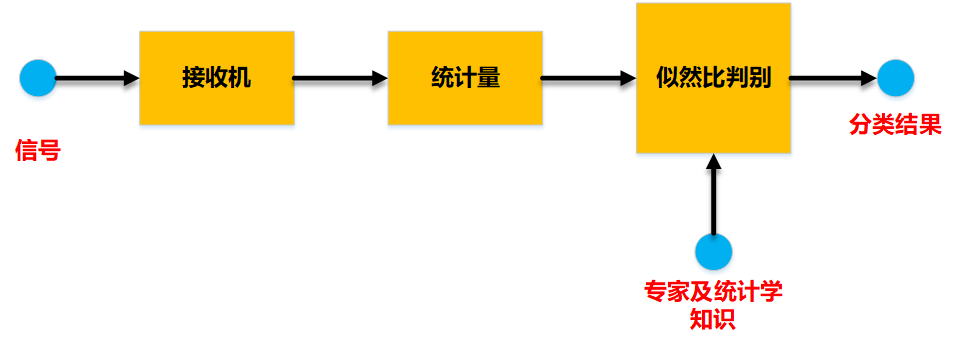
\includegraphics[scale=0.55]{figures/chapter_1/fig_1_0}
	\caption{基于似然比判决理论的调制识别系统框图} \label{sec:fig_1_0}
\end{figure}
对于现有的发展,Kim和Polydoros [4]使用平均似然比检验来识别BPSK和QPSK信号,在信噪比大于$0dB$时,该算法可取得较好的识别效果。
Hwang 和 Polydoros 提出了的两个小信噪比分类规则[9]和正交偏移调制分方法[10]以实现 CPM 信号的识别。
Schreyoegg [5]等人假设QAM信号的幅度和相位彼此大致相互独立,并且使用对数似然函数来使用振幅和相位的联合概率密度函数来识别MQAM信号。 
Wei和Mendel [6]使用复数符号序列的平均似然函数对QAM信号进行分类,并分析了最大似然分类器的渐近行为,当信噪比为5dB时,识别率达到100%。
当可用符号的数量接近无穷大时,分类错误概率接近零,它还给出了参数与错误概率之间的关系。
Baudant等人提出了瑞利衰落信道中FSK信号的调制分类方法[8],解决了衰落信道中的FSK信号调制识别问题。\par
 
似然比决策理论算法的优点是在理论上保证贝叶斯最小误判惩罚准则下分类结果最优,
通过理论分析可以得到分类性能曲线。
但是他同时具有很多局限性:
首先,现有的似然比决策理论算法主要处理符号的同步采样序列,他们需要比模式识别方法更多的先验知识,
这意味着我们需要预先知道信号的载波频率,符号速率和符号时序;
其次,未知参数的似然比分类需要计算复杂的统计表达式,有很大的计算量,很难进行实时处理;
第三,基于似然比决策的算法对模型失配和参数偏差较为敏感,即鲁棒性较差。
似然比函数分类通常被建模为高斯分布,并且诸如信噪比等参数是已知的。
当实际信道噪声为非高斯时,或存在多路径影响、多信号干扰以及SNR参数估计偏差较大时,分类的性能可能会急剧下降。\par
 
\subsection{基于特征提取的统计机器学习方法}

统计机器学习方法基于统计机器学习理论。 
它的基本框架是首先从信号中提取先前选择的特征,然后利用训练好的机器学习模型进行调制识别,包括特征提取子系统和机器学习子系统。基于统计机器学习的调制识别系统框图如图\ref{sec:fig_1_1}所示:\par
\begin{figure}
	\centering
	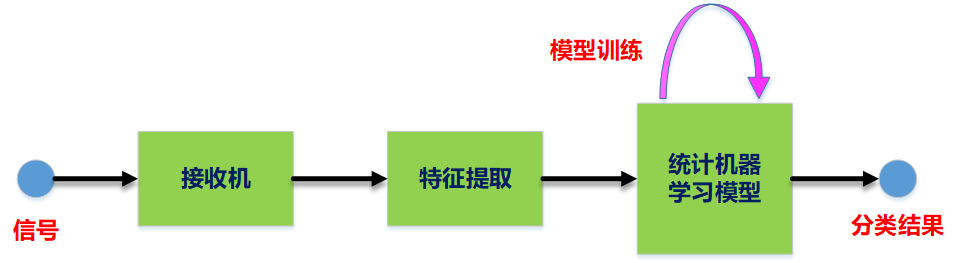
\includegraphics[scale=0.6]{figures/chapter_1/fig_1_1}
	\caption{基于统计机器学习的调制识别系统框图} \label{sec:fig_1_1}
\end{figure}
特征提取子系统主要从未处理信号中提取所需的特征分量,如瞬时频率,瞬时相位和瞬时幅度等。 
模式识别子系统的主要功能是通过特征子系统提取的特征分量对模型进行训练;
模型训练好以后,当需要判别的信号进入该子系统,我们的模型可以对不同的调制信号进行分类。\par

关于数字调制信号识别方法的最早的公开讨论是Liedtke [10], 他提出了一种用于未知调制方法分类的通用分类器。 
该算法可以识别2ASK,2FSK,BPSK,QPSK,8PSK和CW信号,只需要大致了解信号的载波频率和符号率。 Azzouz和ANDI提出了一种算法[11-15],它使用相位的非线性部分,相位的非线性部分的绝对值,
归一化的瞬时振幅和频率等。
调制的标准偏差使用一系列阈值或神经网络分类器来确定参数以识别调制的类型。 后来研究人员在此基础上进行了更多研究 Wong和AK Nandi随后对方法进行了改进[16],
增加了信号的统计参数和训练序列,并且在0dB%时识别率达到了98%。\par

高阶统计量是描述随机过程的高阶统计特性的数学工具,包括高阶矩和高阶累积量,以及高阶周期矩和循环累积量。 Reichert J [19]首次提出使用高阶统计量来识别2ASK,BPSK,2FSK,MSK信号,之后基于高阶统计量的信号识别方法发展迅速。
 Ananthram Swami [20] [21]使用四阶累积量来识别BPSK,4ASK,16QAM和8PSK信号。
当信噪比为10d B时,识别率为95%。 Spooner CM [22]将基于累积量方法的前一种最大化方法打破为四阶例程,提出用6阶循环累积量识别信号,并获得良好的识别效果。
当SNR为9dB时,16QAM总和64QAM的识别率分别为81%和90%。 QPSK和16QAM信号的识别率分别为97%和100%。\par

基于星座的调制识别将调制识别问题转化为形状识别问题。
Bijian [25]详细分析了基于星座图特征的调制识别方法:
通过使用模糊逻辑方法可以很好地恢复原始信号(即接收信号的星座)的特性,
利用贝叶斯最大后验概率准则,对模板进行匹配和判断,
在信噪比大于0dB的情况下,QPSK,8PSK和16QAM分类的正确率可以达到90%。\par
 
对于以上提到的各种分类特征,包括时频统计特征,高阶统计量,星座特征等,
大部分是针对特定类型信号的,而不是对所有的信号都具备一定的辨识能力。
另外,大多数现有的调制识别算法都假定信道是理想的高斯白噪声信道,并且只有少数算法研究了衰落信道。
在实际应用中,无线信道的衰落现象不容忽视,多径效应使得传输信号间存在码间干扰等。
在基于理想高斯白噪声信道环境的识别算法中,信噪比较高时识别性能较好;
当信噪比较低时,算法估计的瞬时包络,相位和频率参数可能会存在较大的误差,使系统的识别性能急剧下降,
并且稳定性差,不能满足实际应用的需求[34]。\par

\subsection{基于深度学习的无线调制识别方法}
深度学习是机器学习中一种基于对数据进行表征学习的方法,最早由Hinton等人于2006年提出。深层神经网络是由一系列层组成网络,其中每一层通常是由已知的具有可调参数和非线性激活函数的线性单元组成,使得深度网络最后可以拟合高度非线性的函数[3]。\par

最近,已有学者证明了利用原始数据学习信号特征进行有监督的调制分类具备一定的可行性[14]。在这种情况下,我们获得的分类性能,超过了传统的基于专家特征的机器学习算法,比如决策树、SVM等。这对于当前的调制识别解决方案提供了一种新的思路,我们可以利用深度学习的方法对现有的调制识别系统进行改进,提高识别的准确率以及鲁棒性,并利用时下深度学习中比较流行的半监督、无监督学习算法,从数据的层面对不同类型的信号进行认知学习。\par

在【】中,Afan提出了一种基于非负约束自编码器的自动调制分类的方法。在无线通信领域,我们具备大量的无标记的数据,而有标记的数据却很少,并且很难获得。为了解决这个问题,XX研究了基于半监督学习的调制识别。在【】中,XX将信号样本的维数降低到一个平滑的较小的空间,相同或相似类型的信号具有较低的距离,而不同类型的信号间隔较大的距离。理想情况下,在这样的空间中,相同或相似类型的例子形成离散且可分离的簇,彼此容易辨别。\par

以上的研究主要是从应用的层面对深度学习的既有方法进行不同领域的迁移应用,并没有提出一定的算法框架或者底层网络结构的改进,而且对于影响性能的因素,算法所能达到的上限,以及将深度学习与传统的调制识别方法结合方面都没有进行一定的研究。因此需要我们对深度学习在调制识别中的应用在算法、框架、应用等层面进行更深入的研究,提高系统的调制识别性能。\par

\section{本文主要工作及内容安排}
从现有的研究成果可以看出,虽然数字通信信号的调制识别算法有很多,
但能够直接利用原始数据对调制信号进行识别的算法还比较少,大多都需要手动进行专家特征提取,
进而训练机器学习模型进行调制识别。
而在实际的非协作通信中,受环境的影响,我们学习的模型在不同的环境中分类性能差别很大,鲁棒性较差。
现有的基于深度学习的调制识别算法,并没有对影响网络性能的因素进行分析,也没能利用过去几十年的研究成果。\par

本文提出了一种基于卷积自编码器和卷积神经网络框架
(Convolutional Autoencoder - Convolutional Neural Network,CAE-CNN)的调制识别算法框架,
并提出了相应框架下的网络训练方法;
提出了对深度特征与传统特征进行融合的算法框架,并对特征融合方式进行了研究;
对影响算法性能的因素进行了研究,讨论了网络的深度、底层结构等对调制识别性能的影响。 \par

本文的具体内容安排如下:

第一章 对无线信号调制识别技术的研究背景和研究现状进行了介绍。\par

第二章 首先介绍了调制信号的基本概念,然后介绍了深度学习的相关理论知识,
为后面基于深度学习的调制识别研究打下理论基础。 \par

第三章 提出了一种CAE-CNN调制识别的算法框架。
首先,介绍了调制信号的生成;
然后,对信号进行了时频域可视化,利用监督方法和无监督方法将信号特征可视化;
接下来,我们将监督方法与无监督方法融合,提出了CAE-CNN的算法;
最后,我们将所提算法的性能进行展示并与传统的方法进行比较。 \par

第四章 提出了一种传统特征与深度特征融合的框架。
首先,介绍了常用的调制识别所用的特征;
然后,对特征融合的相关理论进行概述;接
着,提出了基于LR、DNN以及集成树的融合框架;
最后,对不同特征融合算法的仿真结果进行了相应的理论分析。 \par

第五章 对调制识别的不同网络结构进行了分析验证。
首先,基于CNN网路框架,研究了卷积核数目、大小以及卷基层深度对调制识别的影响;
接下来,研究了网络底层结构(如CLDNN、ResNet等)对调制识别的影响,并对仿真结果进行了理论分析。\par

第六章 总结全文,并对今后的工作进行了展望。\par
